\section{Komplekse tal}
Komplekse tal, er tal der ikke nødvendigvis kan forklares. 
Disse tal indeholder blandt andet tal som $i$, $j$ og $z$, og beskrives med domænet $\mathbb{C}$.
Tallet i bruges blandt andet til at forklare ligningen
\begin{equation}
    \label{eqn:complex}
    x^2=-1
\end{equation}
Med ligningen i \cref{eqn:complex} kan $16i^2=-16$ nu udregnes. 
Med dette kan det konkluderes at $4i$ er løsningen til $x^2=-16$, da $(4i)^2=-16$.
Ligeledes kan ligningen $(x-1)^2=-16$, løses ved $x-1=4i$, hvilket giver at $x=1+4i$.
Derfor kan det konkluderes at alle komplekse tal har en reel del og et imaginær del.

\subsection{Værdier i komplekse tal}
Ligesom almindelige punkter, kan plottes i en graf, kan komplekse tal også plottes.
Betragt følgende eksempel (\cref{fig:C_plot}) fra \cref{lst:c_plot}:
\begin{figure}[h]
    \centering
    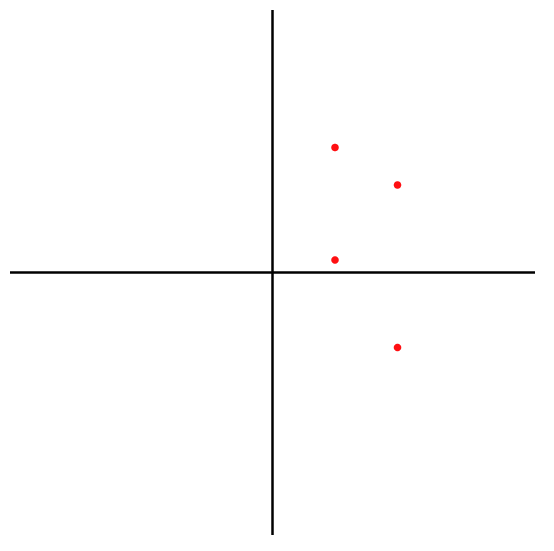
\includegraphics[width=0.5\textwidth]{img/complex_plot.png}
    \caption{Et plot af komplekse tal, i en liste S.}
    \label{fig:C_plot}
\end{figure}
\lstinputlisting[
	language=Python,
    label=lst:c_plot,
    linerange={2-13},
	caption={Python kode til plotte komplekse tal i en graf.\\Koden kan findes i ./labs/fields/complex\_plot.py}
]{labs/fields/complex_plot.py}
Punkterne kan plottes da komplekse tal har en reel værdi samt en imaginær værdi.
Af samme grund kan et komplekst tal også have en længde fra origo, hvilket fremkommer af linjerne 6--10 i \cref{lst:c_plot}.
Dette grundes at på $y$ aksen måles måles punktets imaginære værdi, mens den reele værdi måles på $x$ aksen.
Det sidste er simpel pythagoras.
